% !TeX root = ../main.tex

\chapter{Related work}  \label{chapter:relatedwork}

This chapter presents existing deep learning approaches that have addressed the issue of future frame prediction. These are grouped into three sections depending on the model implementation, namely neural networks, recurrent networks and adversarial networks. The strength, weaknesses and design decisions of these models are briefly discussed, together with a short analysis of the achieved outcomes. Further, it is highlighted how these approaches have influenced the architecture of our final model that is used throughout the evaluation in Chapter \ref{chapter:evaluation}. Aside from that, their results form the baseline in the assessment of our model.


\section{Neural Network Approaches}

First approaches to predict a future images in an image sequence have been done in \parencite{ann} and its follow-up publication \parencite{ann2}.

\begin{figure}[htb]
\centering
\begin{subfigure}{0.5\textwidth}
  \centering
  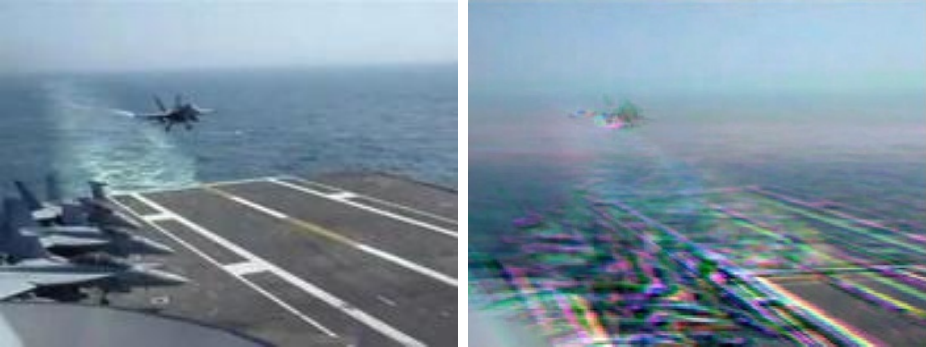
\includegraphics[height=2cm]{figures/related/fighter.png}
  \caption{Fighter dataset}
  \label{fig:aan_samples_fighter}
\end{subfigure}%
\begin{subfigure}{0.5\textwidth}
  \centering
  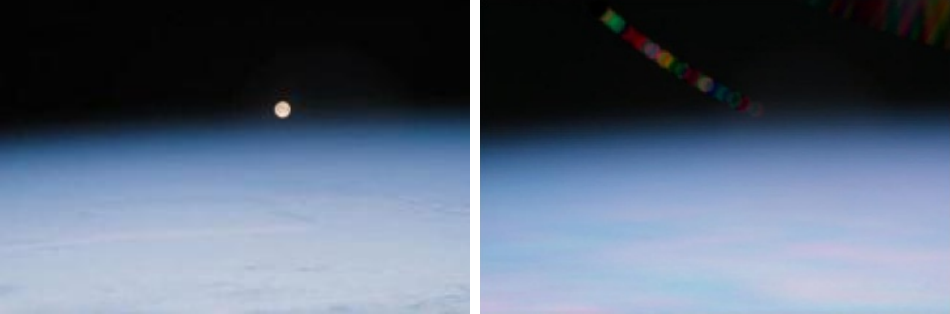
\includegraphics[height=2cm]{figures/related/nasa.png}
  \caption{NASA dataset}
  \label{fig:aan_samples_nasa}
\end{subfigure}
\caption[ANN Frame Prediction]{Single frame predictions using an ANN model with two hidden layers.\\
Left: ground truth target frame. Right: generated prediction.  (From \parencite{ann})}
\label{fig:aan_samples}
\end{figure}




\section{Recurrent Network Approaches}

\begin{figure}[htb]
	\centering
	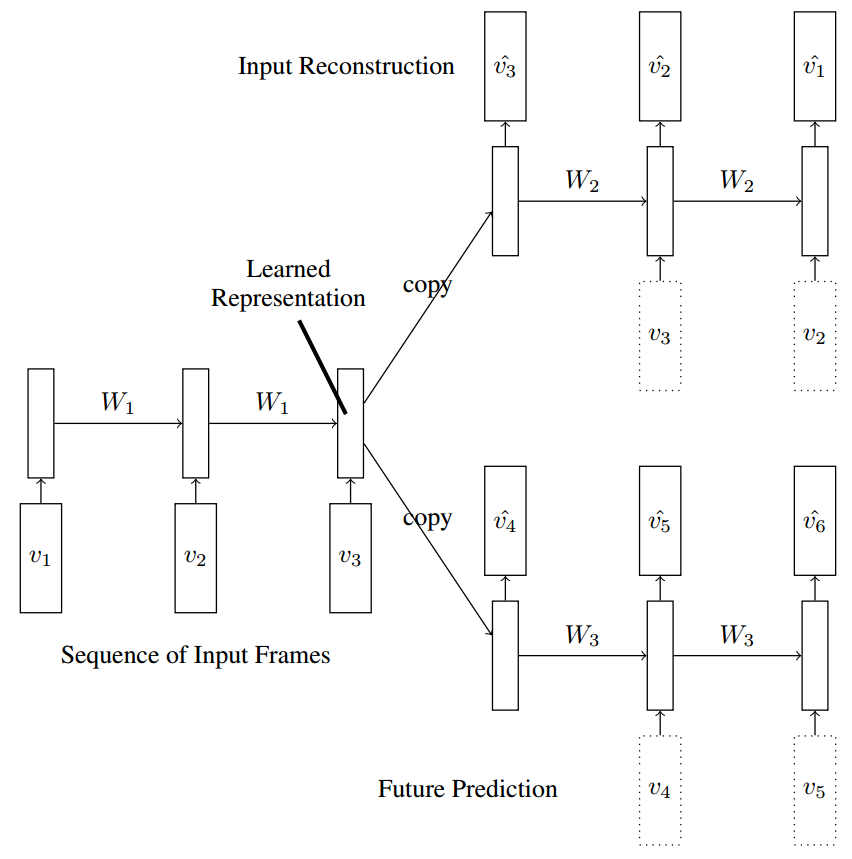
\includegraphics[width=0.5\linewidth]{figures/related/combo_shrinked.png} 
	\caption[Short]{Description.} \label{fig:lstm_combo}
\end{figure}


\begin{figure}[htb]
	\centering
	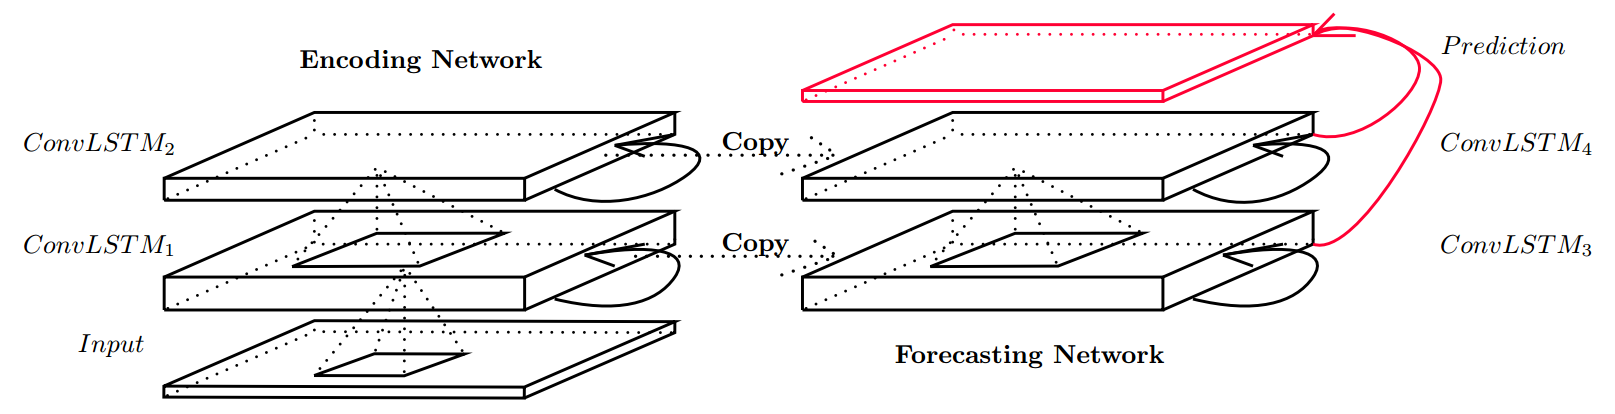
\includegraphics[width=0.8\linewidth]{figures/related/nowcasting_model.png} 
	\caption[Short]{Description.} \label{fig:convlstm_model}
\end{figure}


\begin{figure}[htb]
	\centering
	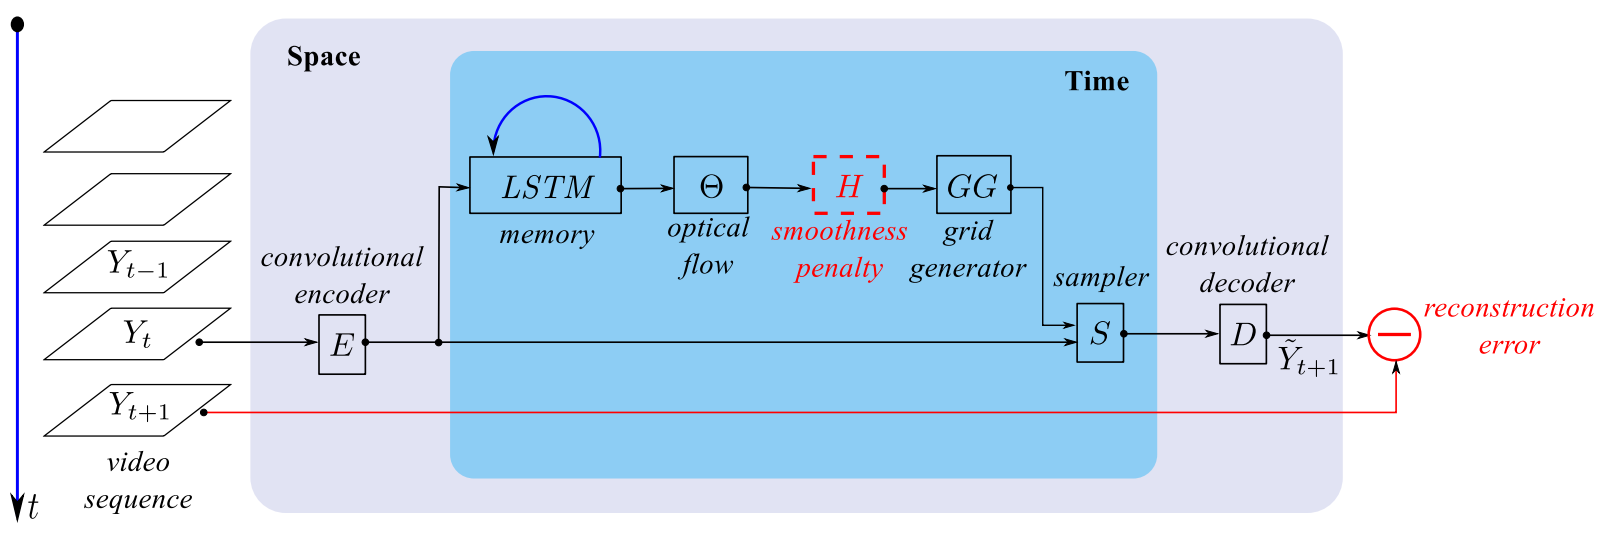
\includegraphics[width=0.8\linewidth]{figures/related/spat_temp_video.png} 
	\caption[Short]{Description.} \label{fig:spatiotemp_model}
\end{figure}


\begin{figure}[htb]
	\centering
	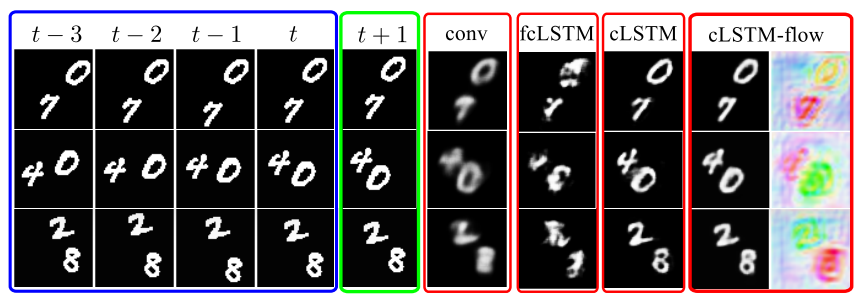
\includegraphics[width=1.0\linewidth]{figures/related/spat_temp_results.png} 
	\caption[Short]{Description.} \label{fig:spatiotemp_results}
\end{figure}


\section{Adversarial Network Approaches}


\begin{figure}[htb]
	\centering
	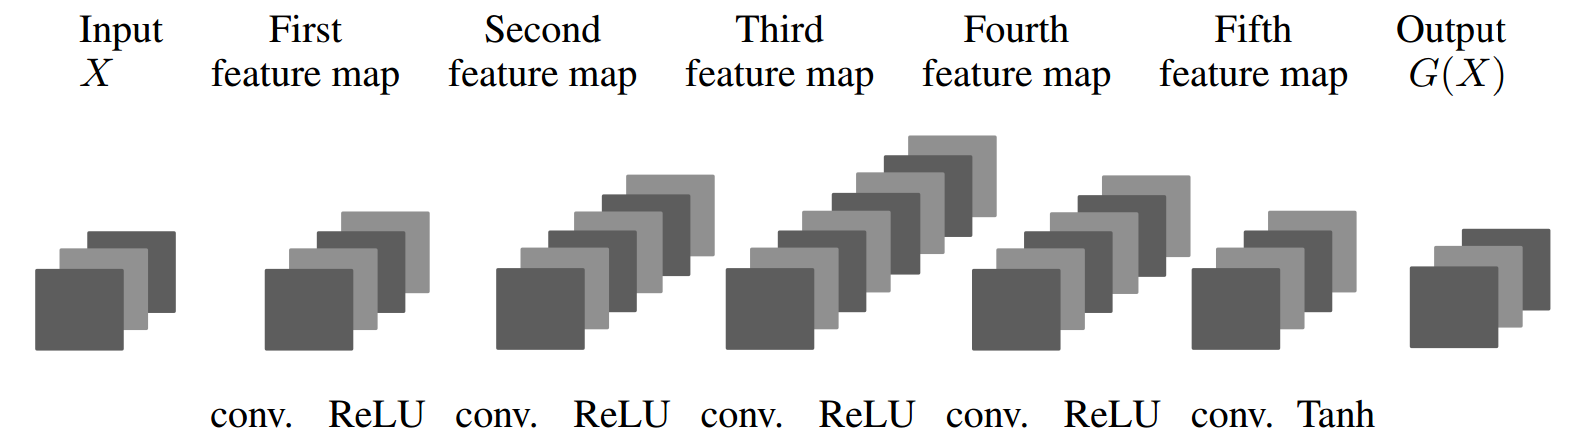
\includegraphics[width=0.8\linewidth]{figures/related/deep_multiscale_generator.png} 
	\caption[Short]{Description.} \label{fig:gan_generator}
\end{figure}


\begin{figure}[htb]
	\centering
	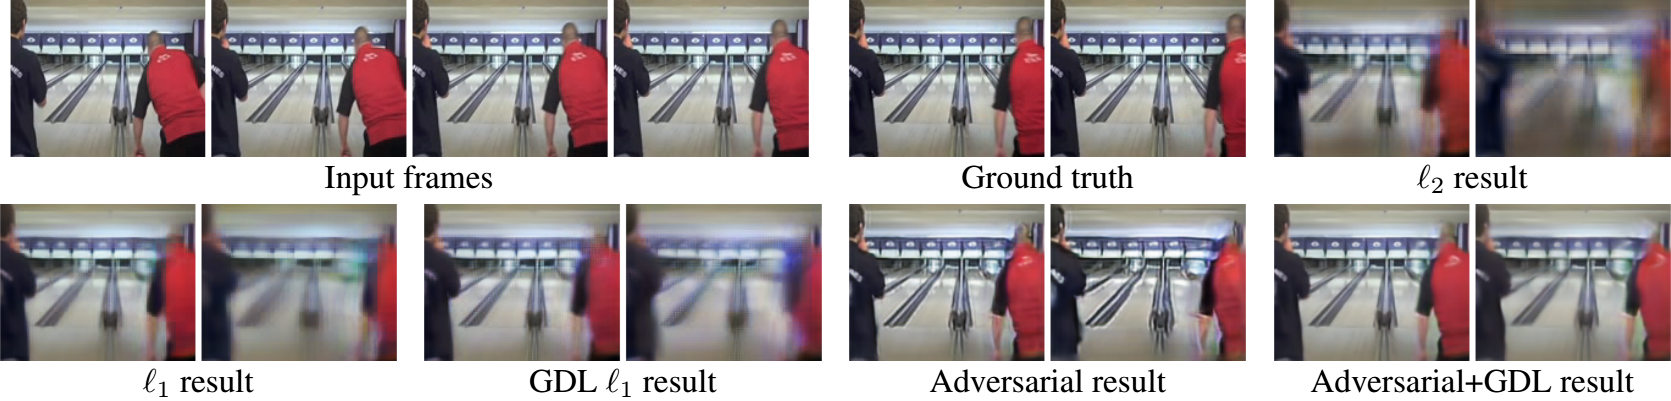
\includegraphics[width=1.0\linewidth]{figures/related/deep_multiscale_samples.png} 
	\caption[Short]{Description.} \label{fig:gan_samples}
\end{figure}





%In \textbf{Chapter \ref{chapter:relatedwork}}, we take a closer look at existing approaches that are suitable for spatio-temporal learning and frame prediction. We briefly discuss their strength and weaknesses, as well as how they have influenced the design decisions regarding the architecture of our final neural network model. Additionally, these presented models build the baselines in our evaluation.